%!TEX root=../document.tex

\section{Ergebnisse}
\label{sec:Ergebnisse}


\subsection{RMI Tutorial}

\subsubsection{Projekt Setup: Java Policy}
Um die RMI APIs zu verwenden, muss die Rechteverwaltung von Java entsprechend konfiguriert werden.
Diese Konfigurationsdatei wird als \textit{Java Policy} bezeichnet und findet sich im konkreten Fall von Mac OS X mit Oracle Java in Folgender Datei:

\texttt{/Library/Java/JavaVirtualMachines/jdk1.8.0\_60.jdk/Contents/Home/jre/lib/security/\\java.policy}

\texttt{jdk1.8.0\_60.jdk} ist dabei die Version der installierten JDK.

Um allen Dateien innerhalb des Benutzerverzeichnisses die entsprechenden Rechte zu geben werden folgende Zeilen hinzugef\"ugt:

\begin{lstlisting}[caption=\"Anderungen in der Java Policy]
grant codeBase "file:/Users/<USERNAME>/-" {
    permission java.security.AllPermission;
};
\end{lstlisting}

\subsubsection{Implementierung}
Es wird das Java RMI Tutorial\cite{rmi-tutorial} mit der Implementierung von Micheal Borko\cite{rmi-tutorial-impl} herangezogen.
Nach der entsprechenden Konfiguration in der Java Policy bereiten sich bei der Ausf\"uhrung mittels den beiden bereits bestehenden Ant-Tasks \texttt{engine} und \texttt{compute} keine weiteren Schwierigkeiten.

Bei der Durchsicht des Tutorialcodes wird ersichtlich, dass es sich dabei bereits um die Implementierung eines Command-Patterns handelt.

\begin{figure}[!h]
	\begin{center}
		\includegraphics[width=0.5\linewidth]{images/Command_design_pattern.png}
		\caption{UML Klassendiagramm des generischen Command Patterns \cite{command-pattern-uml}}
		\label{broker}
	\end{center}
\end{figure}

\texttt{Task} is dabei das Command-Interface und dient dem konkreten Command \texttt{Pi}.
Das vom Server angebotene Remote Object der Klasse \texttt{ComputeEngine} nimmt Tasks (also Kommandos) entgegen, f\"uhrt diesen aus und sendet das Ergebnis zur\"uck an den Client.
Es fungiert somit im Sinne des Command Patterns als Receiver.

\subsection{Berechnung der Euler'schen Zahl}
Um es dem Client auch zu erm\"oglichen die Euler'sche Zahl e zu berechnen wird ein weiter \texttt{Task} mit einem entsprechenden Algorithmus implementiert.
Mathematisch wird dieser durch folgende Summenfunktion ausgedr\"uckt:

\begin{equation*}
\displaystyle\sum_{k=0}^{\infty} \dfrac{1}{k!}
\end{equation*}

Die Java Implementierung wurde einem Stackoverflow Post\cite{euler-stackoverflow} entnommen und in die \texttt{EulerCalculateTast} Klasse eingebaut.

\begin{lstlisting}[style=Java, caption=Funktion zur n\"aeherungweisen Berechnung der Euler'schen Zahl]
public static BigDecimal calculateEuler(int precision) {
    BigDecimal e = BigDecimal.ONE;
    BigDecimal fact = BigDecimal.ONE;

    for(int i=1;i<=precision;i++) {
        fact = fact.multiply(new BigDecimal(i));

        e = e.add(BigDecimal.ONE.divide(fact, new MathContext(10000, RoundingMode.HALF_UP)));
    }
    return e;
}
\end{lstlisting}


\subsection{Asynchrone Berechnung mittels Callbacks}
Um dem Client einen asynchrone Berechnung zur erm\"oglichen wird das Command Pattern um Callbacks\cite{command-pattern-callback} erweitert.
Folgendes UML Klassendiagramm zeigt die Zielstruktur der Applikation:

\begin{figure}[H]
	\begin{center}
		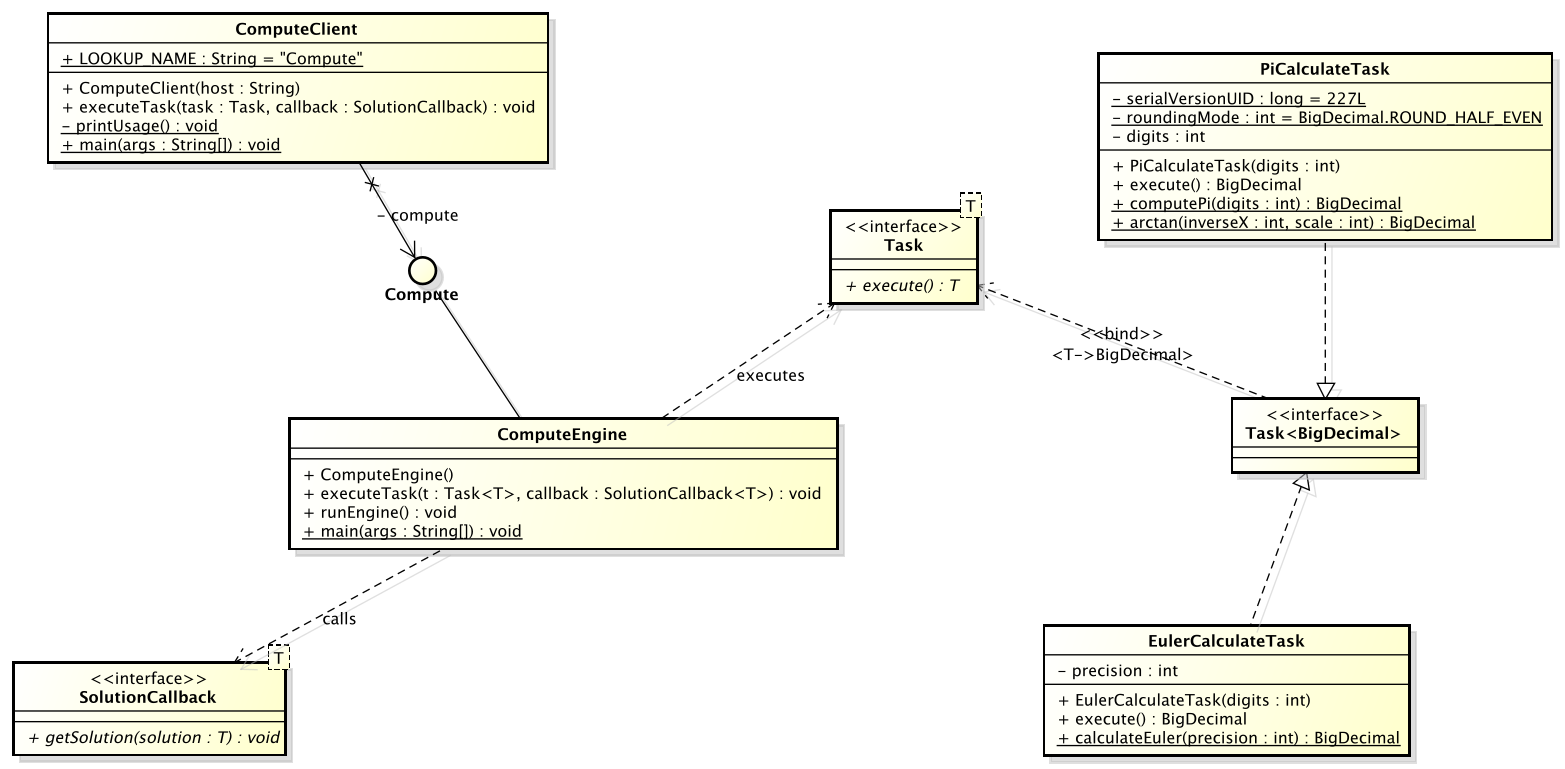
\includegraphics[width=0.8\linewidth]{images/class_diagram.pdf}
		\caption{Applikationsstruktur als UML Klassendiagramm}
		\label{broker}
	\end{center}
\end{figure}

Hier die wichtigsten \"Aenderungen, welche sich durch die Implementierung des Callback ergeben haben.
Es wurde eine \texttt{SolutionCallback} Klasse eingef\"uhrt, welche als Interface zur Implementierung der Callbacks dient.
Genauso wie \texttt{Task} hat sie einen Typparameter, welche den R\"uckgabewert anzeigt.

Der zentrale Kompoenente der Anwendung ist die Klasse \texttt{ComputeEngine} als konkrete Implementierung von \texttt{Compute}.
Ihr wird nun in der \texttt{executeTask} Methode zus\"atzlich zum auszuf\"uhrenden \texttt{Task} auch ein \texttt{SolutionCallback} Objekt \"ubergeben, welches nach der Berechnung mit dem Ergebnis aufrufen wird:
\begin{lstlisting}[style=Java, caption=Funktion zur n\"aeherungweisen Berechnung der Euler'schen Zahl]
public class ComputeEngine implements Compute {

    public ComputeEngine() {
        super();
    }

    public <T> void executeTask(Task<T> t, SolutionCallback<T> callback) {
        new Thread(new TaskExecutor<>(t, callback)).start();
    }

    public void runEngine() {
        if (System.getSecurityManager() == null) {
            System.setSecurityManager(new SecurityManager());
        }
        try {
            String name = "Compute";
            Compute stub =
                    (Compute) UnicastRemoteObject.exportObject(this, 0);
            Registry registry = LocateRegistry.createRegistry(1099);
            registry.rebind(name, stub);
            System.out.println("ComputeEngine bound");
        } catch (Exception e) {
            System.err.println("ComputeEngine exception:");
            e.printStackTrace();
        }
    }

    public static void main(String[] args) {
        ComputeEngine engine = new ComputeEngine();
        engine.runEngine();
    }

    private static class TaskExecutor<T> implements Runnable {
        private Task<T> task;
        private SolutionCallback<T> callback;

        private TaskExecutor(Task<T> task, SolutionCallback<T> callback) {
            this.task = task;
            this.callback = callback;
        }

        @Override
        public void run() {
            T solution = task.execute();
            try {
                callback.getSolution(solution);
            } catch (RemoteException e) {
                e.printStackTrace();
            }
        }
    }
}
\end{lstlisting}

Da das Ziel ist, eine asynchrone (nicht blockierende) Berechnung zu realisieren muss die eigentliche Berechnung, also der Aufruf von \texttt{tast.execute()} jeweils einen eigenen Thread ausgelagert werden.
Hierf\"ur dient die \texttt{TaskExecutor}. Sobald der Client die \texttt{executeTask} Methode von \texttt{ComputeEngine} auruft, erstellt diese einen neuen \texttt{TaskExecutor} starten einen neuen Thread.
An dieser Stelle ist der Methodenaufruf beendet und der Client setzt seine Programmausf\"uhrung fort.
Innerhalb des Threads wird nun die eigentliche Berechnung durchgef\"uhrt und das Ergebnis \"uber den (asynchronen) Callbackaufruf an den Client weitergeleitet.
Das folgende Sequenzdiagram bietet eine \"ubersichtliche Darstellung des Ablaufes.

\begin{figure}[H]
	\begin{center}
		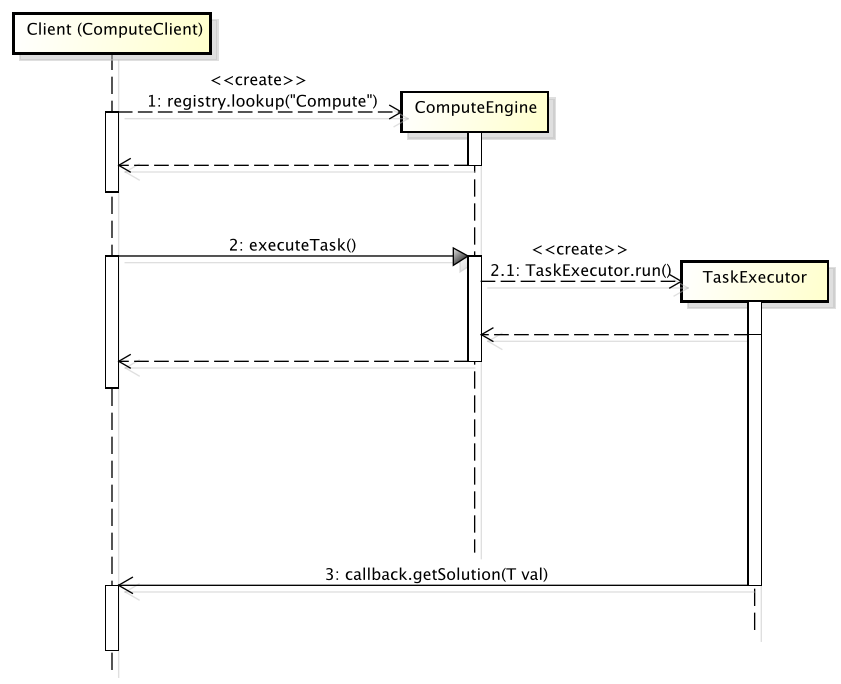
\includegraphics[width=0.6\linewidth]{images/sequence_diagram.pdf}
		\caption{Kommunikationsverlauf zwischen den Komponenten als UML Sequenzdiagramm}
		\label{broker}
	\end{center}
\end{figure}

Bei der Betrachtung des Klassendiagramms wird der Anschein erweckt, dass der Client bei dem Aufruf von \texttt{executeTask} des Remote Objekts das Callback als normales Objekt \"ubergibt.
Wichtig ist dabei jedoch, dass es durch den Aufruf von \texttt{UnicastRemoteObject.exportObject()} in eine Remote Objektreferenz gepackt wird:

\begin{lstlisting}[style=Java, caption=Beispielcode zur asynchronen Ausf\"uhrung einer Berechnung.]
// create callback
SolutionCallback callback = new SolutionCallback() {
    @Override
    public void getSolution(Object solution) throws RemoteException {
        System.out.println(solution);
        // unexport the callback so the program exists smoothly
        UnicastRemoteObject.unexportObject(this, true);
    }
};

// create client
ComputeClient client = new ComputeClient("localhost");

// create task
Task task = new PiCalculateTask(10);

// execute task
client.executeTask(task, (SolutionCallback) UnicastRemoteObject.exportObject(callback, 0));
\end{lstlisting}

Wichtig ist dabei die letzte Zeile, welche das Callback Objekt wieder entfernt und damit der auf entfernte Methodenaufrufe wartet beendet werden kann.

\subsection{Unittests}
\subsubsection{Build Automation}
Da Ant standardm\"a\ss ig nicht f\"ur Dependency Management verwendet werden kann, jedoch f\"ur die sp\"ater beschriebenen Unit Tests einige Libraries zum Einsatz kommen, habe ich mich f\"ur einen Wechsel des Build Systems auf Maven entschieden.
Die Konfiguration von Maven erfolgt ebenfalls mit XMl und ist Ant relativ \"ahnlich, allerdings muss die Projektstruktur etwas abge\"andert werden:

\begin{itemize}
    \item Java Sources: \texttt{src/main/java}
    \item Testcases: \texttt{src/test/java}
\end{itemize}

Als Packagesuffix wird \texttt{klein.rmi} benutzt.

Es stellt sich heraus, dass die Maven Konfigurationsdatei \texttt{pom.xml} durch die vereinheitlichte Packetstruktur sehr simpel und kurz ausf\"allt.
Einige nicht relevanten aber dennoch zwingende Attribute und Elemente wurden weggelassen um Platz zu sparen.

\begin{lstlisting}[style=XML, caption=Maven Konfigurationsdatei]
<project (...)>
    <!-- General configuration options -->
    <groupId>klein.rmi</groupId>
    <artifactId>syt-rmi</artifactId>
    <packaging>jar</packaging>

    <name>SYT 4 RMI</name>

    <!-- Dependencies -->
    <dependencies>
        <dependency>
            <groupId>junit</groupId>
            <artifactId>junit</artifactId>
            <version>4.12</version>
            <scope>test</scope>
        </dependency>
        <dependency>
            <groupId>org.mockito</groupId>
            <artifactId>mockito-core</artifactId>
            <version>2.0.52-beta</version>
            <scope>test</scope>
        </dependency>
    </dependencies>

    <!-- Set language level. Otherwise expressions like lambdas are not allowed -->
    <build>
        <plugins>
            <plugin>
                <groupId>org.apache.maven.plugins</groupId>
                <artifactId>maven-compiler-plugin</artifactId>
                <configuration>
                    <source>1.8</source>
                    <target>1.8</target>
                </configuration>
            </plugin>
        </plugins>
    </build>
</project>
\end{lstlisting}

\subsubsection{Testcases}
Der wichtigste Testcase startet eine \texttt{ComputeEngine}, \"offnet eine Verbindung und f\"uehrt eine Dummyberechnung aus.
Als Callback Objekt kommt ein Spy zum Einsatz, welcher den korrekten Aufruf der Callbackfunktion mit dem erwarteten Ergebnis verifiziert.

\begin{lstlisting}[style=Java, caption=Beispielcode zur asynchronen Ausf\"uhrung einer Berechnung.]
public class ComputeEngineTest {
    @Test
    public void testExecuteTask() throws Exception {
        TestSolutionCallback mockedCallback = mock(TestSolutionCallback.class);

        ComputeEngine engine = new ComputeEngine();
        engine.runEngine();

        ComputeClient client = new ComputeClient("localhost");
        TestTask task = new TestTask();
        client.executeTask(task, (SolutionCallback<Integer>) UnicastRemoteObject.exportObject(mockedCallback, 0));

        // wait for the callback before checking the callback call
        Thread.sleep(700);

        verify(mockedCallback).getSolution(2);
    }

    private static class TestSolutionCallback implements SolutionCallback<Integer> {
        public void getSolution(Integer solution) throws RemoteException { }
    }

    private static class TestTask implements Task<Integer> {
        public Integer execute() {
            // sleep to simulate calculation
            try {
                Thread.sleep(500);
            } catch (InterruptedException e) {
                e.printStackTrace();
            }
            return 2;
        }
    }
}
\end{lstlisting}

\subsection{Arbeitszeit}
\renewcommand{\arraystretch}{1.5}
\begin{table}[H]
	\center
	\begin{tabular}{ | @{\hspace{3mm}} c @{\hspace{3mm}} | @{\hspace{3mm}} l @{\hspace{3mm}} | }
		\hline \textbf{T\"atigkeit} & \textbf{Datum}\\ \hline\hline
		\textbf{Implementierung Aufgabe} & 6.5. 4h\\ \hline
		\textbf{Implementierung + Protokoll} & 11.5. 2h\\ \hline
        \textbf{Protokoll} & 12.5. 3h\\ \hline
	\end{tabular}
	\caption{Arbeitszeitaufzeichnung}
	\label{methoden}
\end{table}
